\begin{frame}{SoCRocket Unique Features}
    \begin{itemize}
        \item RTL counterpart of TLM models are freely available
        \item Completeness of tools and models
        \item Methods for timing analysis
        \item Methods for power analysis
        \item Runtime reconfigurability
        \item \textbf{Enables effective design space exploration}
    \end{itemize}
\end{frame}

\begin{frame}{Configuration Example\footnote{T. Schuster et al. (2014). SoCRocket - A virtual platform for the European Space Agency's SoC development. p.123}}
    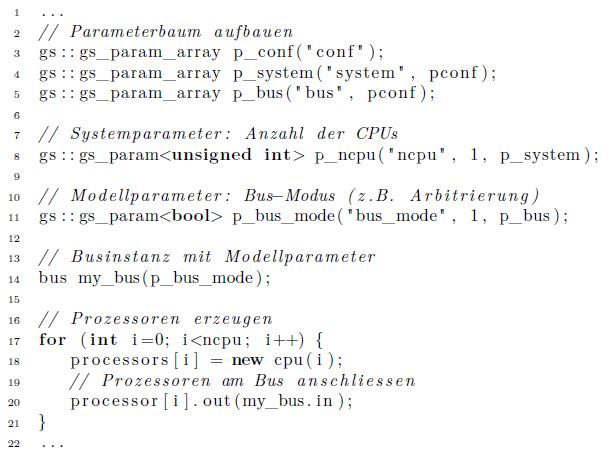
\includegraphics[height=7cm]{pictures/configurationExample.JPG}
\end{frame}

\begin{frame}{SoCRocket Workflow \footnote{L. Fossati et al. (2013). SOCROCKET: A VIRTUAL PLATFORM FOR SOC DESIGN p.3}}
    \centering
    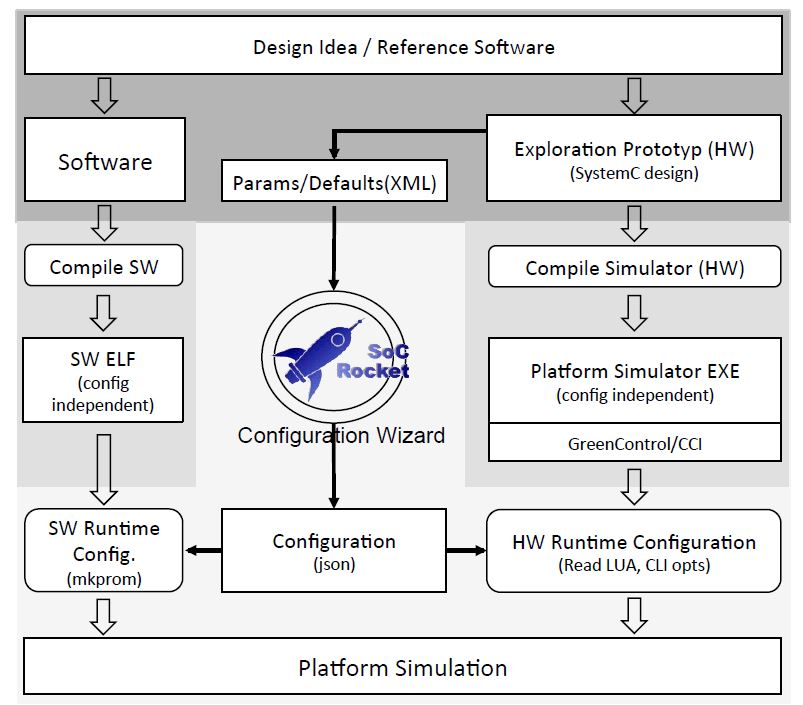
\includegraphics[height=7cm]{pictures/SoCRocket_workflow.JPG}
\end{frame}

\begin{frame}{Leon Processor Overview}
    \begin{block}{Processor Features}
      \begin{itemize}
        \item 32-bit RISC processor
        \item Developed by Aeroflex Gaisler AB
        \item SparcV8 architecture
        \item Special focus on error detection and correction
      \end{itemize} 

    \end{block} \pause
    
    \begin{block}{Field of use}
      \begin{itemize}
        \item Free for educational and scientific applications
        \item Licenseable for commercial applications
        \item Especially suited for aerospace systems
      \end{itemize} 

    \end{block}

\end{frame}

%\begin{frame}{Leon Processor TLM Model \footnote{T. Schuster et al. (2014). SoCRocket - A virtual platform for the European Space Agency's SoC development. p.78}}
%   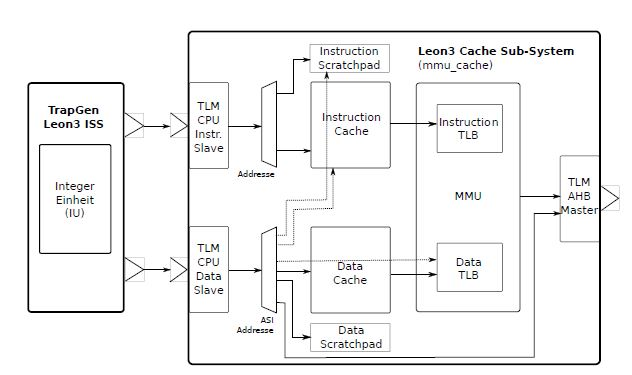
\includegraphics[height=7cm]{pictures/leonTlmModel.JPG}
%\end{frame}


